\section{Apache Spark with Docker}\label{s:apache-spark-with-docker}

\subsection{Pull Image from Docker
Repository}

We use a Docker image from Docker Hub:
(https://hub.docker.com/r/sequenceiq/spark/) This repository contains a
Docker file to build a Docker image with Apache Spark and Hadoop Yarn.

\begin{lstlisting}
docker pull sequenceiq/spark:1.6.0
\end{lstlisting}

\subsection{Running the Image}

In this step, we will launch a Spark container.

\subsubsection{Running interactively}

\begin{lstlisting}
docker run -it -p 8088:8088 -p 8042:8042 -h sandbox sequenceiq/spark:1.6.0 bash
\end{lstlisting}

\subsubsection{Running in the
background}

\begin{lstlisting}
docker run -d -h sandbox sequenceiq/spark:1.6.0 -d
\end{lstlisting}

\subsection{Run Spark}

After a container is launched, we can run Spark in the following two
modes: 1) yarn-client and 2) yarn-cluster. The differences between the
two modes can be found here:
https://spark.apache.org/docs/latest/running-on-yarn.html

\subsubsection{Run Spark in Yarn-Client
Mode}

\begin{lstlisting}
spark-shell --master yarn-client --driver-memory 1g --executor-memory 1g --executor-cores 1
\end{lstlisting}

\subsubsection{Run Spark in Yarn-Cluster
Mode}

\begin{lstlisting}
spark-submit --class org.apache.spark.examples.SparkPi --master yarn-client --driver-memory 1g --executor-memory 1g --executor-cores 1 $SPARK_HOME/lib/spark-examples-1.6.0-hadoop2.6.0.jar
\end{lstlisting}

\subsection{Observe Task Execution from Running Logs of SparkPi}

Let us observe Spark task execution by adjusting the parameter of
SparkPi and the Pi result from the following two commands.

\begin{lstlisting}
spark-submit --class org.apache.spark.examples.SparkPi --master yarn-client --driver-memory 1g --executor-memory 1g --executor-cores 1 $SPARK_HOME/lib/spark-examples-1.6.0-hadoop2.6.0.jar 10
\end{lstlisting}

\begin{lstlisting}
spark-submit --class org.apache.spark.examples.SparkPi --master yarn-client --driver-memory 1g --executor-memory 1g --executor-cores 1 $SPARK_HOME/lib/spark-examples-1.6.0-hadoop2.6.0.jar 10000
\end{lstlisting}

\subsection{Write a Word-Count Application with Spark RDD}

Let us write our own word-count with Spark RDD. After the shell has been
started, copy and paste the following code in console line by line.

\subsubsection{Launch Spark Interactive Shell}

\begin{lstlisting}
spark-shell --master yarn-client --driver-memory 1g --executor-memory 1g --executor-cores 1
\end{lstlisting}

\subsubsection{Program in Scala}

\begin{lstlisting}
val textFile = sc.textFile("file:///etc/hosts")
val words = textFile.flatMap(line => line.split("\\s+"))
val counts = words.map(word => (word, 1)).reduceByKey(_ + _)
counts.values.sum()
\end{lstlisting}

\subsubsection{Launch PySpark Interactive Shell}

\begin{lstlisting}
pyspark --master yarn-client --driver-memory 1g --executor-memory 1g --executor-cores 1
\end{lstlisting}

\subsubsection{Program in Python}

\begin{lstlisting}
textFile = sc.textFile("file:///etc/hosts")
words = textFile.flatMap(lambda line:line.split())
counts = words.map(lambda word:(word, 1)).reduceByKey(lambda x,y: x+y)
counts.map(lambda x:x[1]).sum()
\end{lstlisting}

\subsection{Docker Spark Examples}

\subsubsection{K-Means Example}

First we need to pull the image from the Docker Hub :

\begin{lstlisting}
docker pull sequenceiq/spark-native-yarn
\end{lstlisting}

It will take sometime to download the image. Now we have to run docker
spark image interactively.

\begin{lstlisting}
docker run -i -t -h sandbox sequenceiq/spark-native-yarn /etc/bootstrap.sh -bash
\end{lstlisting}

This will take you to the interactive mode.

Let's run a sample KMeans example. This is already built with Spark.

Here we specify the data data set from a local folder inside the image
and we run the sample class KMeans in the sample package. The sample
data set used is inside the sample-data folder. Spark has it's own
format for machine learning datasets. Here the kmeans\_data.txt file
contains the KMeans dataset.

\begin{lstlisting}
./bin/spark-submit --class sample.KMeans --master execution-context:org.apache.spark.tez.TezJobExecutionContext --conf update-classpath=true ./lib/spark-native-yarn-samples-1.0.jar /sample-data/kmeans_data.txt
\end{lstlisting}

If you run this successfully, you can get an output as shown here.

\begin{lstlisting}
Finished iteration (delta = 0.0)
Final centers:
DenseVector(0.15000000000000002, 0.15000000000000002, 0.15000000000000002)
DenseVector(9.2, 9.2, 9.2)
DenseVector(0.0, 0.0, 0.0)
DenseVector(9.05, 9.05, 9.05)
\end{lstlisting}

\subsubsection{Join Example}

Run the following command to do a sample join operation on a given
dataset. Here we use two datasets, namely join1.txt and join2.txt. Then
we perform the join operation that we discussed in the theory section.

\begin{lstlisting}
./bin/spark-submit --class sample.Join --master execution-context:org.apache.spark.tez.TezJobExecutionContext --conf update-classpath=true ./lib/spark-native-yarn-samples-1.0.jar /sample-data/join1.txt /sample-data/join2.txt
\end{lstlisting}

\subsubsection{Word Count}

In this example the wordcount.txt will used to do the word count using
multiple reducers. Number 1 at the end of the command determines the
number of reducers. As spark can run multiple reducers, we can specify
the number as a parameter to the programme.

\begin{lstlisting}
./bin/spark-submit --class sample.WordCount --master execution-context:org.apache.spark.tez.TezJobExecutionContext --conf update-classpath=true ./lib/spark-native-yarn-samples-1.0.jar /sample-data/wordcount.txt 1
\end{lstlisting}

\subsection{Interactive Examples}

Here we need a new image to work on. Let's run the following command.
This will pull the necessary repositories from docker hub, as we don't
have most of the dependencies related to it. This can take a few minutes
to download everything.

\begin{lstlisting}
docker run -it-p 8888:8888 -v $PWD:/cloudmesh/spark --name spark jupyter/pyspark-notebook
\end{lstlisting}

Here you will get the following output in the terminal.

\begin{figure}[htbp]
\centering
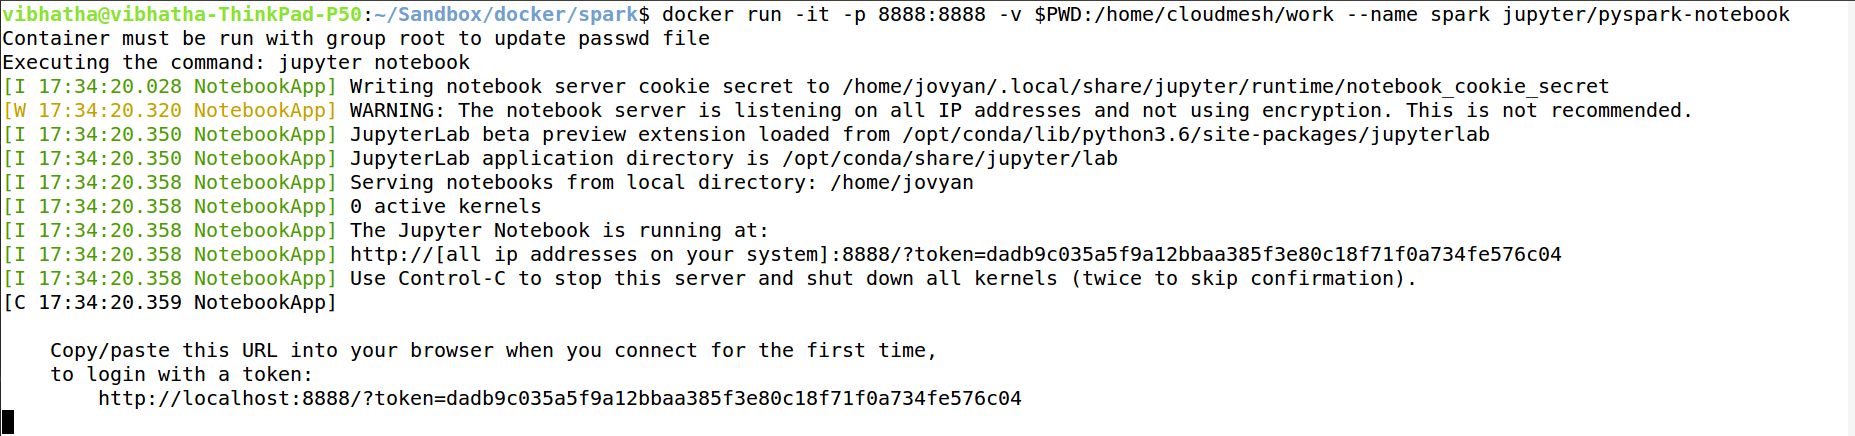
\includegraphics[width=0.7\textwidth]{images/docker-spark-jupyter.png}
\caption{Terminal Output}
\end{figure}

Please copy the url shown at the end of the terminal output and go to
that url in the browser.

You will see the following output in the browser, (Use Google Chrome)

\begin{figure}[htbp]
\centering
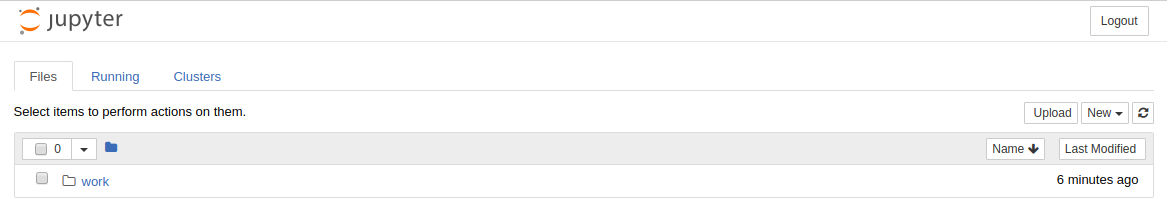
\includegraphics[width=0.7\textwidth]{images/docker-spark-jup-1.png}
\caption{Jupyter Notebook in Browswer}
\end{figure}

First navigate to the work folder. Let us create a new python file here.
Click python3 in the new menu.

\begin{figure}[htbp]
\centering
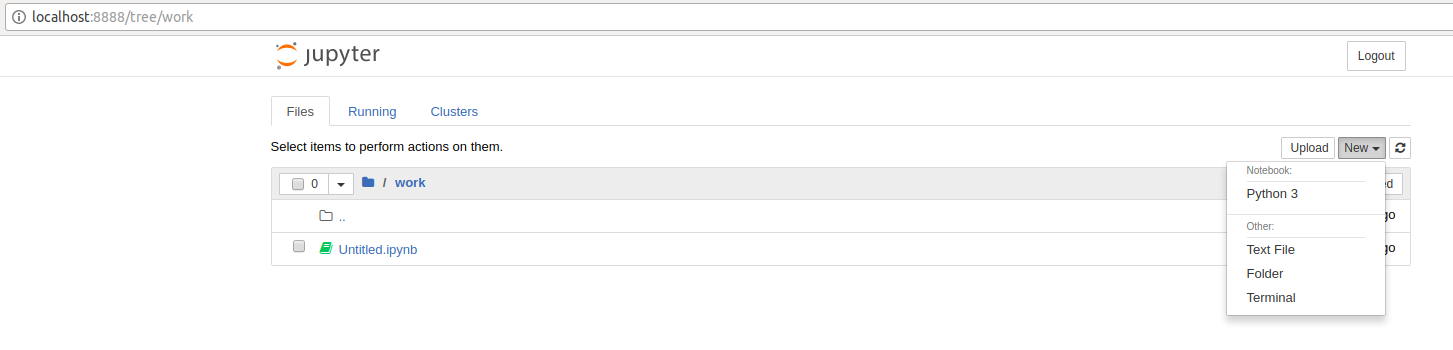
\includegraphics[width=0.7\textwidth]{images/docker-spark-jup-2.png}
\caption{Create a new python file}
\end{figure}

Now add the following content in the new file. In Jupyter notebook, you
can enter a python command or python code and press

\begin{lstlisting}
SHIFT + ENTER
\end{lstlisting}

This will run the code interactively.

Now let's create the following content.

\begin{figure}[htbp]
\centering
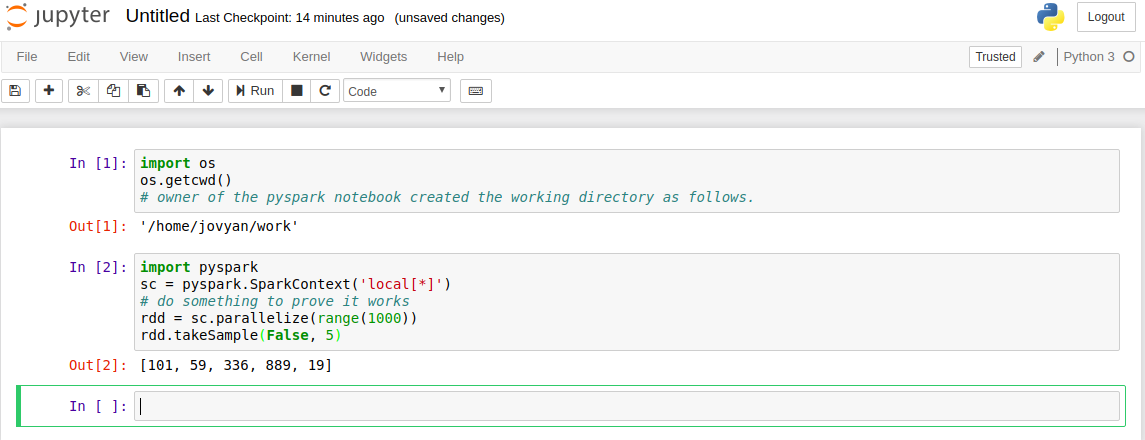
\includegraphics[width=0.7\textwidth]{images/docker-spark-jup-3.png}
\caption{Create a new python file}
\end{figure}

Now let us do the following.

In the following stage we configure spark context and import the
necessary files.

\begin{figure}[htbp]
\centering
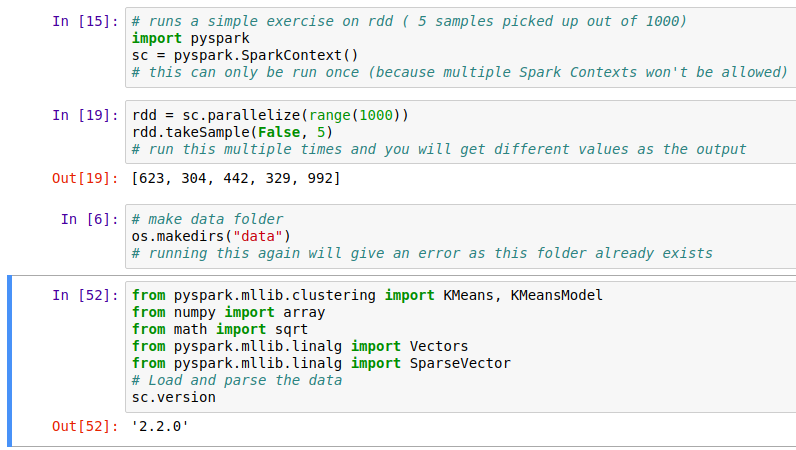
\includegraphics[width=0.7\textwidth]{images/docker-spark-tut-1.png}
\caption{Initial Spark Program}
\end{figure}

Next stage we use sample data set by creating them in form of an array
and we train the kmeans algorithm.

\begin{figure}[htbp]
\centering
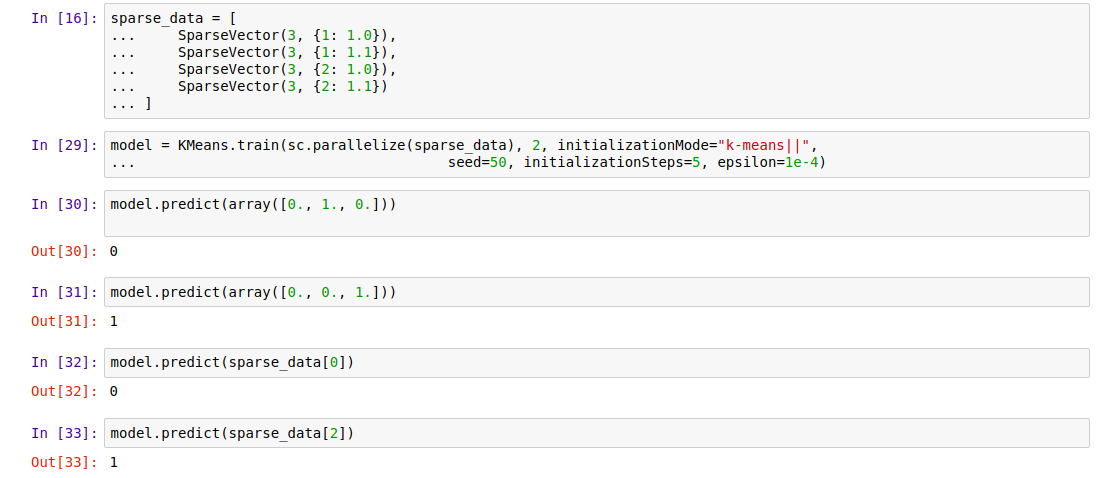
\includegraphics[width=0.7\textwidth]{images/docker-spark-tut-4.png}
\caption{Train KMeans}
\end{figure}

In the final stage we put sample values and check the predictions on the
cluster. In addition to that feed the data using SparseVector format and
we add the kmeans initialization mode, the error margin and the
parallelization. We put the step size as 5 for this example. In the
previous one we didn't specify any parameters.

The predict term predicts the cluster id which it belongs to.

\begin{figure}[htbp]
\centering
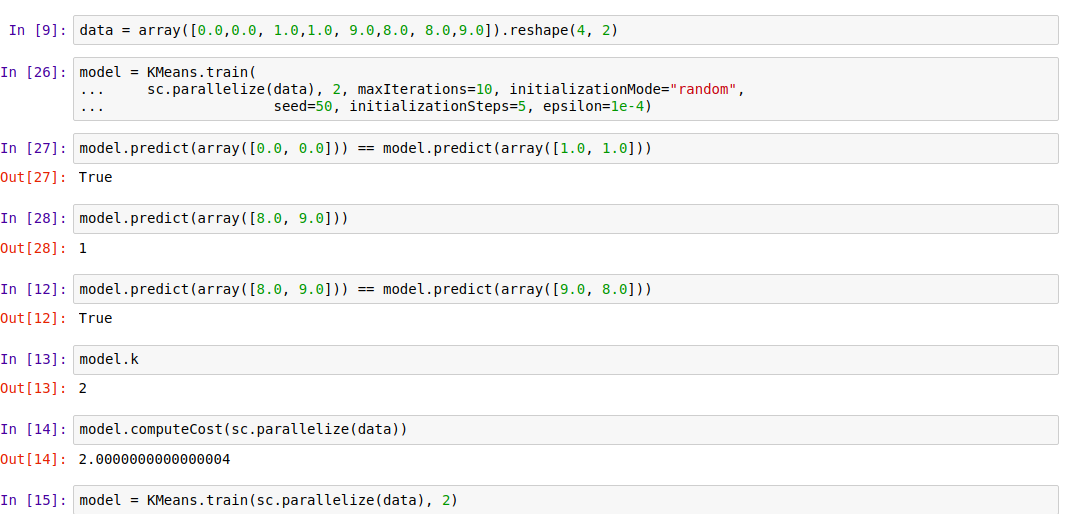
\includegraphics[width=0.7\textwidth]{images/docker-spark-tut-5.png}
\caption{Predict KMeans Clusters-1}
\end{figure}

Then in the following way you can check whether two data points belong
to one cluster or not.

\begin{figure}[htbp]
\centering
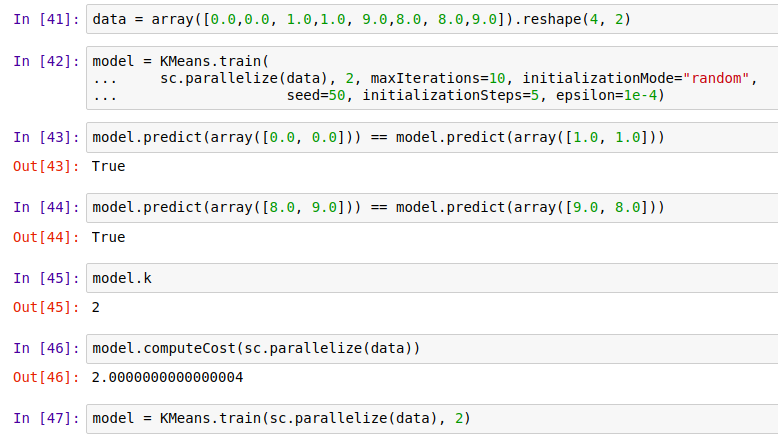
\includegraphics[width=0.7\textwidth]{images/docker-spark-tut-2.png}
\caption{Predict KMeans Clusters-2}
\end{figure}

\begin{figure}[htbp]
\centering
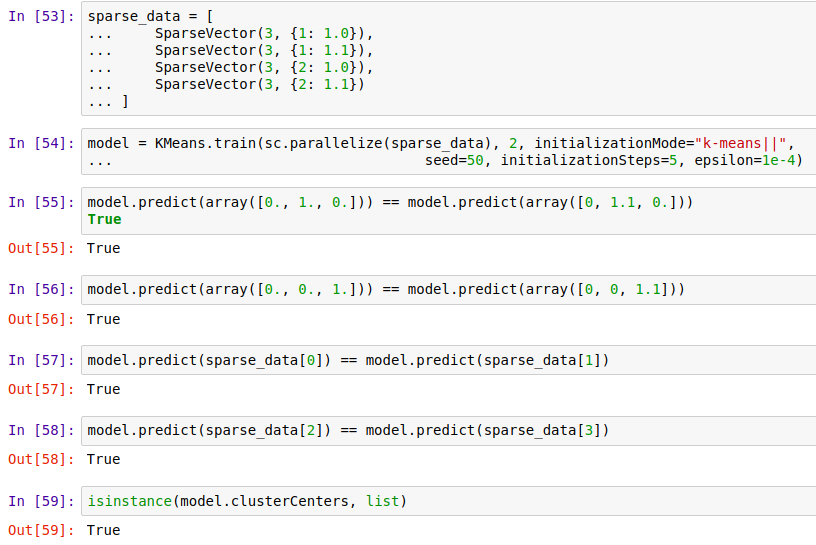
\includegraphics[width=0.7\textwidth]{images/docker-spark-tut-3.png}
\caption{Predict KMeans Clusters-3}
\end{figure}

\subsubsection{Stop Docker Container}

\begin{lstlisting}
docker stop spark
\end{lstlisting}

\subsubsection{Start Docker Container
Again}

\begin{lstlisting}
docker start spark
\end{lstlisting}

\subsubsection{Remove Docker Container}

\begin{lstlisting}
docker rm spark
\end{lstlisting}